\section*{Background}

Understanding complicated networks of biomolecular entities and interactions is essential to solving contemporary problems in modern biology, especially in computational domains such as systems biology\textasciitilde{}\cite{hanahan2011hallmarks}.
Networks of bio-molecular interactions are represented as graph models referred to as \emph{pathways}.
Pathways are curated subsets of a theoretical graph of all known biomolecular entities and events that occur on the cellular level, and a given pathway usually represents a particular biological process, such as mitosis, that is relevant within a given research context.

Pathways are modeled as labeled graphs of entities, relationships, and meta-data. For example, Figure \ref{fig:kvik} shows a typical representation of a pathway as a human curated node-link diagram, where nodes are biological entities and edges represent interactions between them.
An entity is a component of a pathway such as a gene, a gene produce (such as a protein), a complex of proteins, a small biomolecule, or even another pathway.
Edges between vertices in this graph can be directed or undirected, can involve multiple entities in one relationship, and can represent a wide range of biological relationships.
Meta-data can include external information such as experimental data, as well as the \emph{provenance} of the information related to a particular entity or relationship.
Provenance is typically a list of records, such as publications, that reflects the collective history of research related to a given entity or relationship.
Provenance is essential to the field of bioinformatics, as the ``ground truth'' related to any given entity is not immutable, and can be derived from a potentially large and evolving history of research.

\begin{figure}[htb]
  \centering
  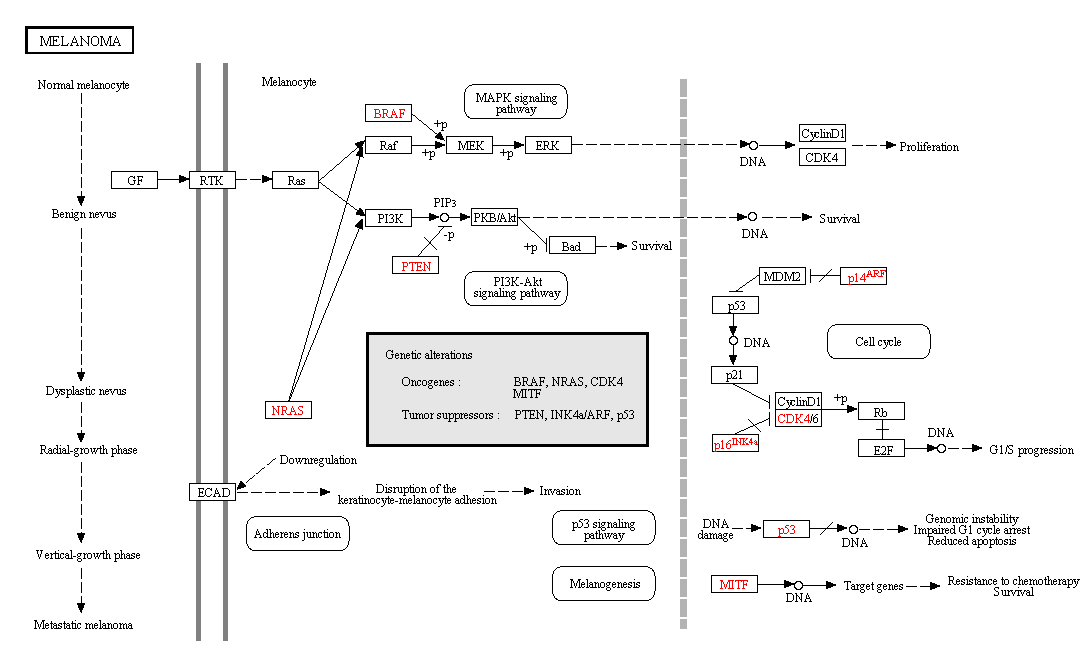
\includegraphics[width=\linewidth]{figures/kegg2}
  \caption{\label{fig:kvik} A view of a typical KEGG diagram. From~\cite{Fjukstad2014kvik}.}
\end{figure}

Researchers who work with pathway data are confronted with a number of challenges.
Pathway files may contain hundreds or thousands of entities that are connected by a wide variety of relationship types.
For instance, the \emph{BioPax} specification \hl{citation! http://www.biopax.org/release/biopax-level3-documentation.pdf} contains a ``Transport'' class, which is one of four types of ``Conversion'', which in turn is one of five different types of ``Interaction'', which, finally, is one of four types of ``Entity''.
The \emph{BioPax} schema is itself a reflection of the complexity of information that can exist within bio-chemical pathway datasets.

Participants in a pathway -- genes, proteins, and other molecules within a cell -- can act as inputs or outputs to multiple interactions, and the set of relationships between biochemical interactions inherently includes feedback loops and other complex relationships.
Importantly, reactions and other interactions can have a ``cascading'' effect, where one interaction will inhibit or promote the effect of another.
Molecular activation pathways also have an inherently dynamic quality, which can limit the utility of static (i.e., non-interactive) graph representations \cite{kitano2002systems}.
Understanding these complex and dynamic relationships while also enabling researchers to see higher order patterns is a significant challenge to modern bioinformatics research \cite{saraiya2005visualizing}.

Pathway diagrams are used in two contexts: for the presentation of results, and as an active (and interactive) part of the process of data analysis.
In the presentational sense, pathway diagrams can contextualize a set of biological processes within a cell, and in these contexts will often show the location of cellular membranes and other large cellular structures to help provide a frame of reference for the viewer.
Ideally, a pathway diagram --~when used in a presentational context -- allows a viewer to efficiently understand a complex set of biological relationships.
While pathway diagrams may be useful for presenting and contextualizing a set of results in a research or educational context, they are also an important part of \emph{in situ} analyses.

For example, metabolic activation networks are of critical importance to cancer researchers, who hope to understand -- and potentially disrupt -- malignant cycles of uncontrolled cellular growth, replication, and mediated cell death \cite{cairns2011regulation}.
Effective cancer drug development involves determining how proteins and complexes that are affected by a drug in turn affect important cellular pathways.
In this domain, the ``downstream'' consequences of a particular drug effect are especially important \cite{luo2003targeting}.
Stem-cell researchers can also use pathways as an active part of their research, where the goal is generally to precipitate a desired cellular differentiation into specific cell types \cite{reya2001stem}.
In these contexts, understanding the complex relationships that are encoded in pathway data is paramount.

In the last two decades, as the availability of large stores of data to researchers has increased, analyses that involve hundreds or thousands of genes and gene products have become common.
When analyzing such large and complex data, visual representations can be essential, and in many cases static, non-interactive, representations will fail to adequately convey the dynamic nature of a pathway.
The complexity and amount of information that needs to be incorporated in given diagram can also make static representations cluttered and difficult to interpret.
Thus, modern applications in these domains employ a wide variety of interactive visualization techniques to allow a user to effectively explore and analyze pathway data.

Developing and designing effective visual analytics applications requires a detailed understanding of the visual analysis tasks that will be performed by a user, and the ``user'' in this case is a biological researcher in the midst of some analysis relevant to their domain.
User tasks can thus be designed and understood best through a in-depth understanding of the nature of information needed by the researcher in the course of their analyses.
Some of these tasks may not be known \emph{a priori} and may be exploratory in nature, where an ideal visualization of pathway data could reveal important new insights to a researcher.
A comprehensive understanding of tasks performed by domain researchers in a typical analysis is essential to the design and implementation of an effective visual analytics application.

In this work, we present a description and analysis of tasks and requirements related to the analysis of biological pathway data.
Tasks were derived from interviews with several domain experts in biology.
After an introduction to the structure and content of pathway data, we describe the task taxonomy that was constructed from these interviews.
We also review visual representations of pathway data in the context of our requirements, along with a brief discussion of existing tools which implement those visual representations.
Finally, avenues of future research are considered, along with a brief summary of lessons learned from domain experts.

\subsection*{Biological Pathway Visualization}

Pathway models are an important concept in biological research\textasciitilde{}\cite{cairns2011regulation, luo2003targeting, reya2001stem}.
Visualization techniques and applications are important tools for researchers who work with complex data, and biological pathways are an active area of visualization research.

A number of surveys exist that describe the large number of existing tools for biological network visualization \cite{Suderman2007tools,pavlopoulos2008survey,Gehlenborg2010omics}.
In this paper we highlight some of the more prominent existing tools and techniques that provide support for the tasks described in our taxonomy.
However, this paper is not intended to be a complete survey of biological visualization techniques and applications.
Existing techniques included in this paper include the following: \textit{ChiBe}\textasciitilde{}\cite{Babur2010chibe}, \textit{Entourage}\textasciitilde{}\cite{Lex2013entourage}, \textit{Reactome Pathway Browser}\textasciitilde{}\cite{croft2014reactome}, \textit{VisAnt}\textasciitilde{}\cite{hu2004visant}, \textit{MetaViz}\textasciitilde{}\cite{bourqui2007metabolic}, \textit{VitaPad}\textasciitilde{}\cite{holford2005vitapad}, and \textit{BioFabric}\textasciitilde{}\cite{Longabaugh2012biofabric}.

Node-link diagrams are the nearly-universal choice of visual representation used in existing applications (exceptions to this rule include Biofabric\textasciitilde{}\cite{Longabaugh2012biofabric}).
Cytoscape \cite{cytoscape} is a popular graph visualization application which was originally designed for biological data, and offers many sophisticated plug-ins that have been developed by the research community, including Cerebral\cite{Barsky2008cerebral} and RenoDoI\cite{Vehlow2015}.
However, node-link representations are one of several ways to visualize graph data, and there are alternative visualization techniques which can be applied to pathway data.
For instance, research has shown that matrix visualization techniques outperform node-link diagrams for higher level group based tasks\cite{Ghoniem2004,Henry2007}.
While these matrix techniques are not as effective for certain tasks (such as path-tracing), linked views and hybrid techniques exist, such as NodeTrix\textasciitilde{}\cite{NodeTrix2007}, which combine node-link and matrix representations.

\subsubsection*{Pathway Data Formats}

Pathway data can be stored in a varitey of file formats which capture the underlying structure of pathway data.
In particular, \textit{BioPAX}\textasciitilde{}\cite{demir2010biopax}, \textit{KEGG}\textasciitilde{}\cite{kanehisa2000kegg} and \textit{SBML} \cite{Hucka2003} are the most popular file standards for storing the complex graph data structures inherent in pathway data.

MORE TO DO HERE

\section*{Methods}

\subsection*{Interviews}

Interviews were conducted with seven domain experts in biology, each of whom works with pathway data in some form.
Those interviewed included one tenured professor, three assistant professors, one researcher at a cancer research institution, one postdoctoral research associate, and one masters student in bioinformatics.
Interviews were loosely structured, but interview questions were designed to elicit a detailed understanding of the tasks performed by the researcher in the course of a typical analysis, as well as an understanding of the type and structure of data that each researcher worked with.
Each researcher also presented their views on the utility of pathway data and of pathway diagrams in general.
We have developed a taxonomy based on these interviews.
In addition, we describe examples of how each task category is addressed by current biological visualization applications and techniques.

\section*{Results and Discussion}

Biological pathways are represented as weighted, directed, labeled graphs which can include hyper-edges and compound nodes.
While existing task taxonomies describe tasks related to the visual analysis of graphs in general\textasciitilde{}\cite{Ahn2014, Pretorius2014}, the analysis of pathways in the context of biology reveals several important graph-analytic tasks that other works have not described in detail.
This taxonomy refines and extends the existing set of tasks associated with the visual analysis of network data in general

\subsection*{Attributes}

The low-level identification of nodes, edges, and their attributes is an essential component of the visual analysis of any graph representation.
In the context of biology, the attributes of a node or edge can itself be a complex object.
Here, we highlight three forms of attribute data that are particularly relevant to biological contexts: multivariate data from experimental results, provenance data, and measures of uncertainty.
We also discuss the need for the integration of external data sources.

\subsubsection*{Multivariate Attributes}

\paragraph*{Description}

The entities within a biological pathway can contain many attributes that reflect the state of that entity in a given context, such as an experimental condition.
In interviews, researchers stressed the importance of being able to visualize potentially complex experimental data while viewing a pathway.
For example, each member of a particular pathway can be associated with gene expression levels across several different experimental conditions, and each of these conditions can include an additional temporal dimension\textasciitilde{}\cite{Barsky2008cerebral}.
In this example, each node would be associated with at least three additional dimensions (experimental condition, expression level, and time).
This multivariate data can also apply to relationships between entities, such as when one gene is up-regulated or down-regulated by another gene under different experimental conditions.

\paragraph*{Existing Approaches and Techniques}
